\section{バージョン管理システムとは?}

\begin{frame}[t,fragile]{バージョン管理システムの必要性}
  \begin{itemize}
    \setlength{\itemsep}{1em}
  \item 広く行われている「ファイル管理」
    \begin{itemize}
    \item ファイル名・ディレクトリ名による管理

      (日付、人名、バージョン番号など)
    \item 手書きのログファイルによる記録
    \end{itemize}
  \item 問題点
    \begin{itemize}
    \item 記録を付け忘れる、記録を間違う、不完全な記録
    \item 人により命名規則がばらばら
    \item コンピュータ間でコピーを繰り返すと、どれを修正したか、どれが新しいか分からなくなる
    \item 同じバージョンを元に、別の人が独立に修正を行ってしまう

      (バージョンの分岐)
    \end{itemize}
  \end{itemize}
\end{frame}

\begin{frame}[t,fragile]{ありがちなパターン}
  \vspace*{-1.8em}
  \begin{center}
    \resizebox{0.93\textwidth}{!}{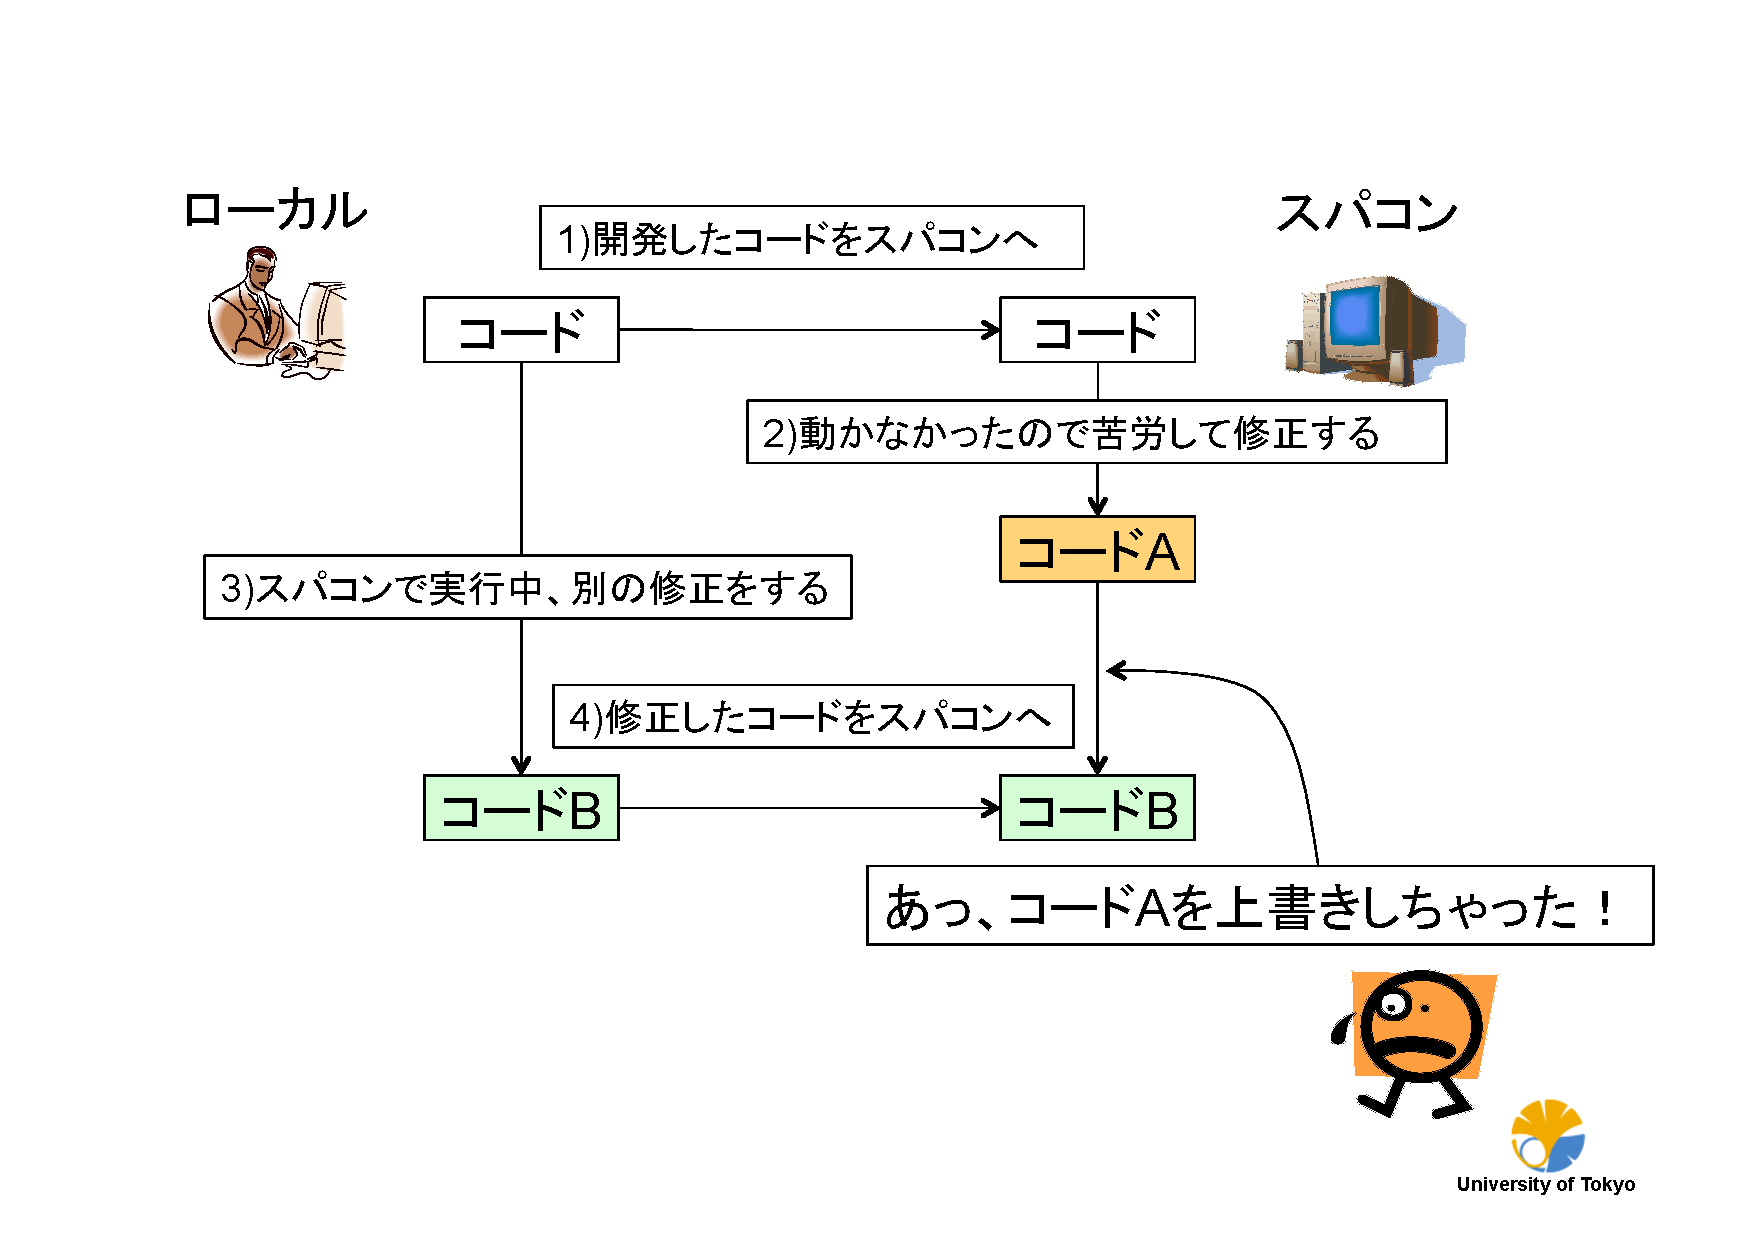
\includegraphics{image/vcs-bad.pdf}}
  \end{center}
  \vspace*{-2em}
  {\footnotesize (渡辺2013)}
\end{frame}

\begin{frame}[t,fragile]{バージョン管理システム(Version Control System)とは?}
  \begin{itemize}
    \setlength{\itemsep}{1em}
  \item ファイルの履歴をデータベース(リポジトリ)で一括管理するシステム
    \begin{itemize}
    \item 全ての修正履歴(差分)を保存
    \item 更新毎に一意なバージョン番号(リビジョン)を付与
    \item 任意のバージョン間の比較が可能
    \item もともとはプログラムのソースコードのためのシステム
    \item それ以外のファイル(例えば TeX ファイル)管理にも使える
    \end{itemize}
  \item チーム・分散環境での作業をサポート
    \begin{itemize}
    \item ネットワーク経由でファイルを check out/check in
    \item 複数箇所から同時に更新した場合に衝突を回避するしくみ
    \item ブランチ・マージ・タグの管理
    \item 一人で使っても複数人で使っても超便利
    \item 超優秀な(かつ超まじめな)秘書のようなもの (しかもタダ)
    \end{itemize}
  \end{itemize}
\end{frame}

\begin{frame}[t,fragile]{バージョン・ブランチ・マージ}
  \begin{center}\resizebox{!}{0.8\textheight}{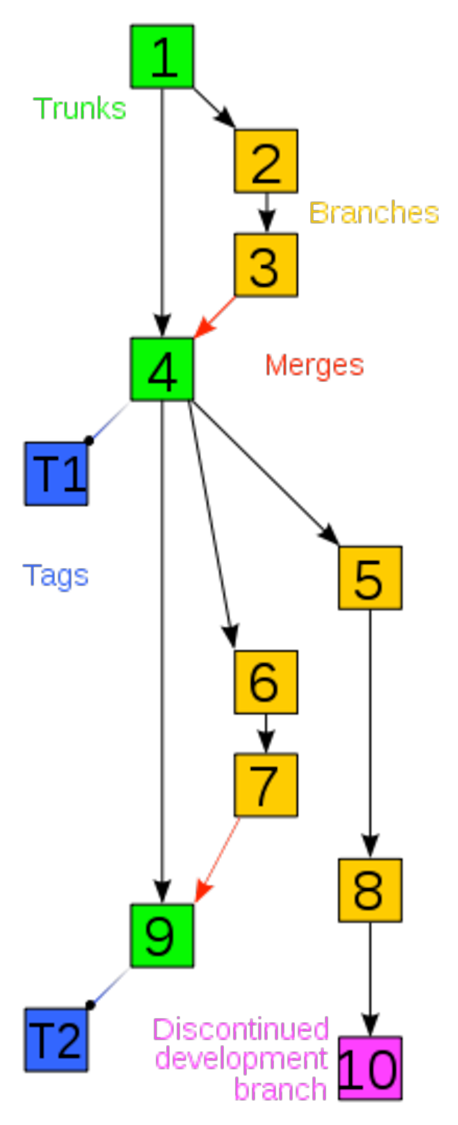
\includegraphics{image/revision.pdf}}\end{center}
\end{frame}

\begin{frame}[t,fragile]{バージョン管理を使うと}
  \vspace*{-1.8em}
  \begin{center}
    \resizebox{1.0\textwidth}{!}{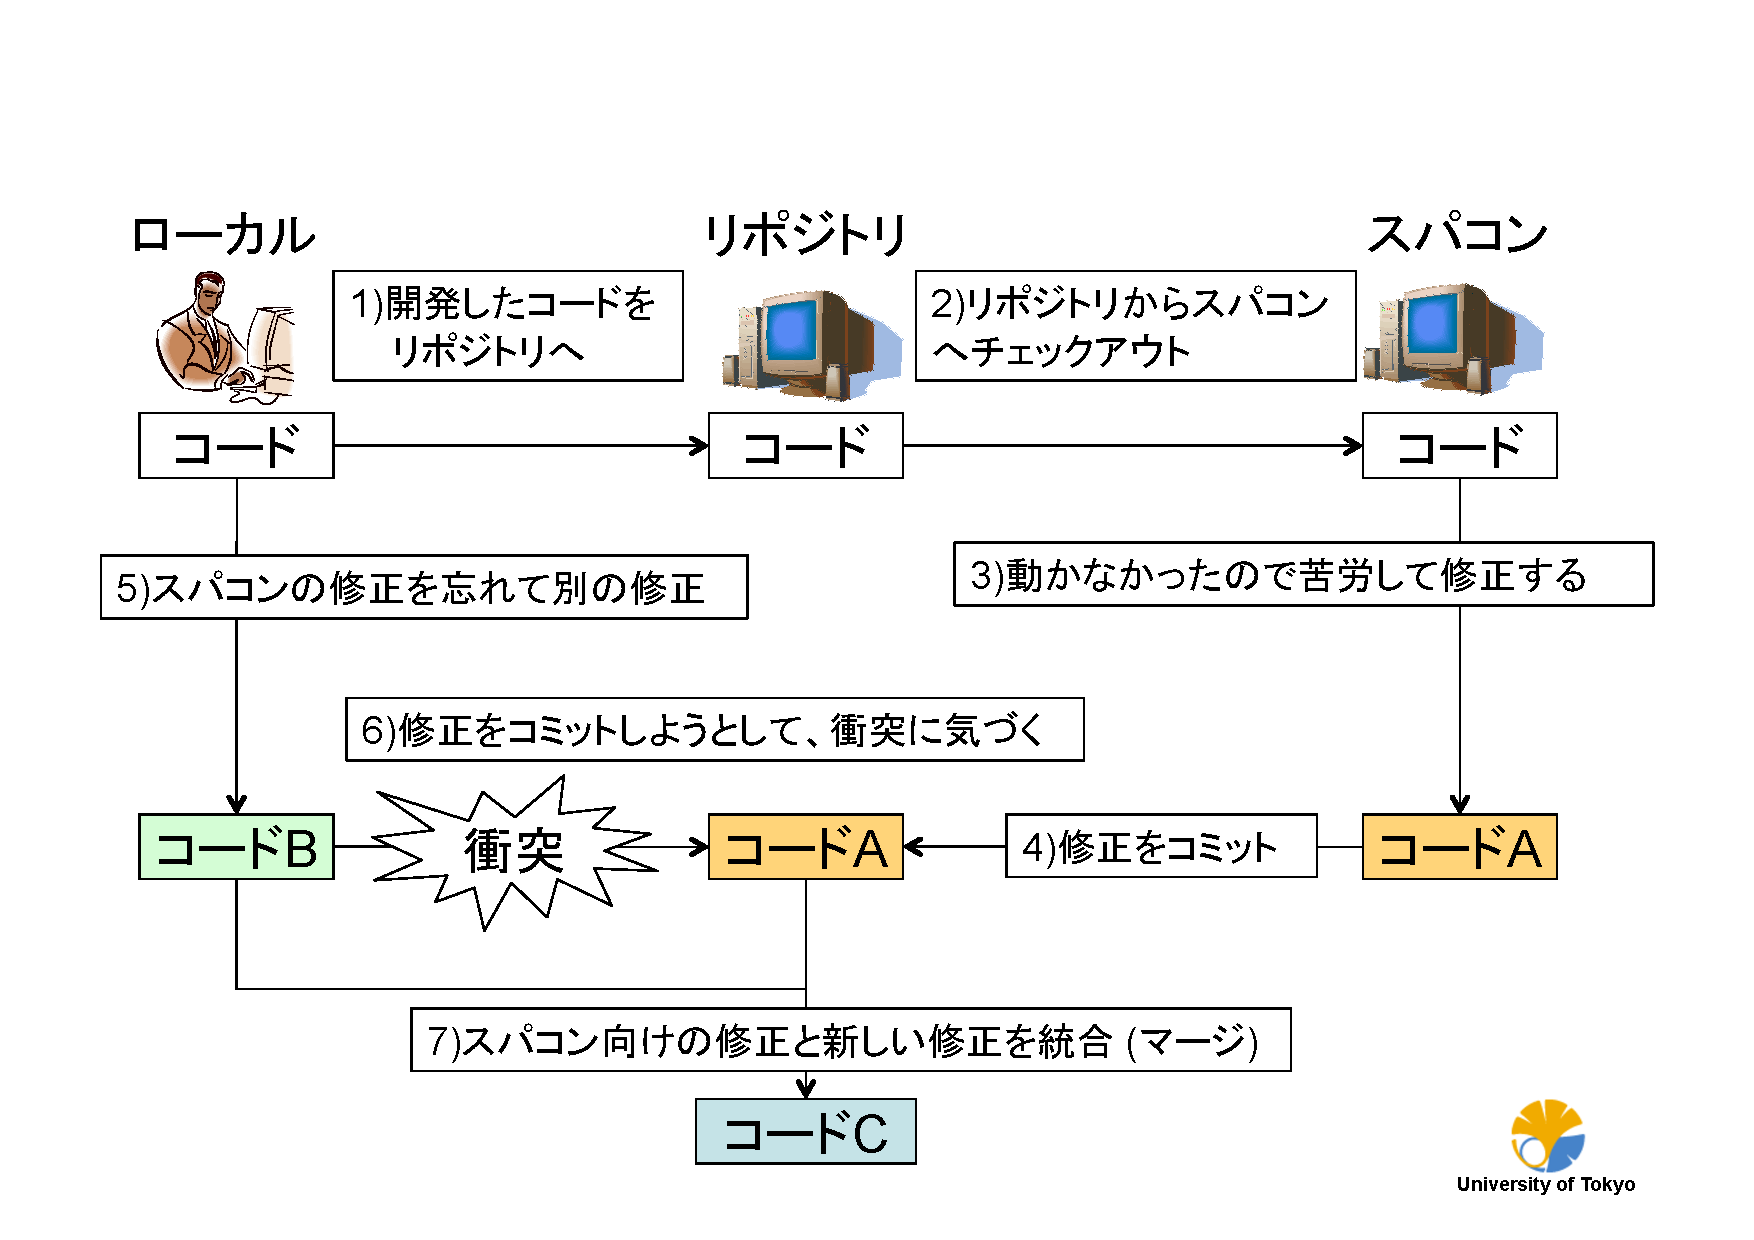
\includegraphics{image/vcs-good.pdf}}
  \end{center}
  \vspace*{-2em}
  {\footnotesize (渡辺2013)}
\end{frame}

\begin{frame}[t,fragile]{diff と patch}
  \begin{itemize}
    \setlength{\itemsep}{1em}
  \item {\tt diff}: 2つのテキストファイルの差分を出力するコマンド
    \begin{itemize}
    \item ファイル全体を保存するよりコンパクト
    \item 変更点を確認しやすい
      
      {\tt \$ \underline{diff -u file1.txt file2.txt > file.diff}}
    \end{itemize}
  \item {\tt patch}: {\tt diff}コマンドが生成した差分をファイルに適用するユーティリティー
    \begin{itemize}
    \item もとのファイルと差分から変更後のファイルを生成できる

      {\tt \$ \underline{patch < file.diff}}
    \end{itemize}
  \end{itemize}
\end{frame}

\begin{frame}[t,fragile]
  \frametitle{実習: diff \& patch (1)}
  \begin{itemize}
    %\setlength{\itemsep}{1em}
  \item 単一ファイルの例
\begin{lstlisting}
$ cp prologue.txt prologue-orig.txt
$ vi prologue.txt # prologue.txtを編集

$ diff -u prologue-orig.txt prologue.txt > prologue.diff
$ less prologue.diff # prologue.diffの中身を見てみる

$ mv prologue-orig.txt prologue.txt
$ patch < prologue.diff
$ less prologue.txt # prologue.txtの中身を確認
\end{lstlisting}
  \end{itemize}
\end{frame}

\begin{frame}[t,fragile]
  \frametitle{実習: diff \& patch (2)}
  \begin{itemize}
    %\setlength{\itemsep}{1em}
  \item ディレクトリ全体を扱う例
\begin{lstlisting}
$ cp -r vcs vcs.orig
# vcsの中のファイルを編集(ファイルの削除や追加も可)

$ diff -urN vcs.orig vcs > vcs.diff
$ less vcs.diff # vcs.diffの中身を見てみる

$ rm -rf vcs
$ mv vcs.orig vcs
$ patch -p0 < vcs.diff
# vcsの中身を確認
\end{lstlisting}
  \item diff と patch で差分の管理は可能になるが, 履歴は別に管理してお
    かなければならない
  \end{itemize}
\end{frame}
